\section{Temperature anomalies}
Written by Aubry Cholleton.
\subsection{Introduction}

Temperature anomalies correspond to the difference between a temperature record/average
and the average of the temperatures recorded in the same conditions during a given reference period.
For example, it is possible to compute the temperature anomaly in Switzerland in April 2014, by
computing the average of the average temperature in April from 1960 to 2000 and subtracting it to the
average temperature in April 2014. Temperature anomalies are much more useful than absolute temperature values since
 they are an objective indicator of climate change in the world.
Some datasets of temperature anomalies already exist, but they offer a
low resolution (5x5 degrees) which is not enough to deal with small countries like Switzerland.
Also we wanted to be able to choose a reference period ourselves when computing anomalies and to perform some statistics and classification of unusual events, so for these reasons we decided to implement our own algorithm.

\subsection{Algorithms}

Our algorithm can be used to compute anomalies and various statistics from the NOAA/NCDC dataset, and both spatial and temporal aggregation
can be performed. Additionally the algorithm classify the anomalies into 5 categories : NORMAL, HIGH, LOW, VERY HIGH, VERY LOW.
The algorithm is not specific to temperature and can be reused for other type of records, nevertheless anomalies are particularly relevant in the case of temperatures.\\
\\It is possible to configure the output of the algorithm using several parameters.

\begin{table}[H]
\begin{tabular}{|l|l|}
\hline
\textbf{Parameter}      & \textbf{Description}                                                                                                                                                                                                                                                                                                       \\ \hline
Input path              & Folder which contains files of raw data from NOAA/NCDC dataset.                                                                                                                                                                                                                                                            \\ \hline
Output path             & Folder which will contains the results of the algorithm.                                                                                                                                                                                                                                                                   \\ \hline
Temporal granularity    & \begin{tabular}[c]{@{}l@{}}By setting this parameter to 1, anomalies will be computed by day.\\ By setting it to 2, anomalies will be computed by month.\end{tabular}                                                                                                                                                      \\ \hline
Grid resolution X       & \begin{tabular}[c]{@{}l@{}}Allows to aggregate data spatially, setting this parameters to values \textgreater0 \\ will produce a gridded dataset of anomalies, where every cell have a \\ size of X*Y degrees. \\ Setting these values to 0 will compute anomalies per weather station\\ without aggregation.\end{tabular} \\ \hline
Grid resolution Y       &                                                                                                                                                                                                                                                                                                                            \\ \hline
First year of reference & \begin{tabular}[c]{@{}l@{}}Define the bounds of the period to take as a reference when\\ computing the anomalies and the statistics. \\ Overlaps with the period to analyze are possible.\end{tabular}                                                                                                                     \\ \hline
Last year of reference  &                                                                                                                                                                                                                                                                                                                            \\ \hline
First year to analyse   & Define the bounds of the period to analyse                                                                                                                                                                                                                                                                                 \\ \hline
Last year to analyse    &                                                                                                                                                                                                                                                                                                                            \\ \hline
\end{tabular}
\caption{Parameters of the algorithm}
\end{table}
The output of the algorithm consist a list of files, each file corresponding to one time slot (day or month).
Each line of a file has the following structure :

\begin{table}[H]
\resizebox{\textwidth}{!}{%
\begin{tabular}{|l|l|l|l|l|l|l|l|}
\hline
\textbf{Content} & Date & X top-left cell corner & \begin{tabular}[c]{@{}l@{}}Y top-left\\  cell corner\end{tabular} & Anomaly & \begin{tabular}[c]{@{}l@{}}Anomaly for \\ maximum \\ temperature\end{tabular} & \begin{tabular}[c]{@{}l@{}}Anomaly for \\ minimum \\ temperature\end{tabular} & Event  strength \\ \hline
\textbf{Example} & 20120529 & +16002 & -155998 & -13 & -11 & -10 & VERYCOLD \\ \hline
\end{tabular}
}
\caption{Output of the algorithm}
\end{table}
The algorithms consists of 6 chained MapReduce phases:

\begin{description}
\item[Per reference station statistics] \hfill \\
The mapper reads the temperature and geo-localisation values from the NOAA dataset, and checks the quality code of the records. It drops records with a low quality. One reducer per station then ensures that the station is up during the whole reference period and that there are enough records. If this is the case, it will compute the average, minimum and maximum temperature over both time slots (days or months) of the reference period and finally average them over the whole period for a given month or day. It will also compute the 90-percentile and the 10-percentile for maximum, minimum and average values, which will be used later to classify anomalies.
\item[Per station statistics] \hfill \\
The mapper reads the temperature and geo-localisation values from the NOAA,dataset, and checks the quality code of the records. It drops records with a low quality. One reducer per station will then compute the mean of these values over each time slots of the period to analyse.
\item[Build grid for reference period]
\item[Build grid for period to analyze] \hfill \\
These 2 mapreduce phases simply aggregate the data of the previous steps in a grid. Each coordinate is converted to the top-left corner coordinate of the cell it belongs to and one reducer per cell then averages the various statistics we have in this given cell.
\item[Compute anomalies] \hfill \\
For every cell and for every time slot this phase computes the anomaly by computing the difference between the reference values and the new values. Classification is also performed at this step. If the maximum values do not belong to the 90-percentile of the maximum values during the reference period, the event is classified as HOT. If both the maximum values AND the minimum values are above the 90-percentile of their distribution during the reference period, the event is classified as VERY HOT. The same principle is applied with COLD events using the 10-percentile of the reference distributions of minimum values.
\item[Output results] \hfill \\
During this final step, the data is split into the desired output format (one file per year/month/day ...).
\end{description}

\subsection{Post processing and Visualization}

Once the results are obtained, and before they are displayed, we try to fill the gaps between the stations using linear interpolation in a python script. This step is skipped with a gridded dataset, which already spans the whole territory.
Depending on the map background which is used, a python script transforms the projection of the points from EPSG4326 to EPSG4857.
Finally it is necessary to export the (gridded) data we get from the algorithm to a format which is easy do display. After several attempts with images, we have finally chosen the GeoJson format, which allows to display stations as coloured points, and cells of the gridded temperature anomalies dataset as polygons.
The temperature anomalies can be loaded as a layer on a leaflet map, together with some controls to select the time slot (day/month) and the type of the displayed anomalies (mean values, maximum values, minimum values).
The cells classified as extreme by the algorithm have a higher opacity and a stronger border, a check box allow the user to display only squares classified as extreme.

\subsection{Interpretation}
The algorithm was run with various parameters. In the final visualization, we chose to build a gridded dataset (2x2 degrees cells) of anomalies from 1997 to 2013, with the period 1980-2005 as a reference. Such a computation takes about one hour on our cluster for the temporal granularity of both day and month.
\begin{figure}[H]
   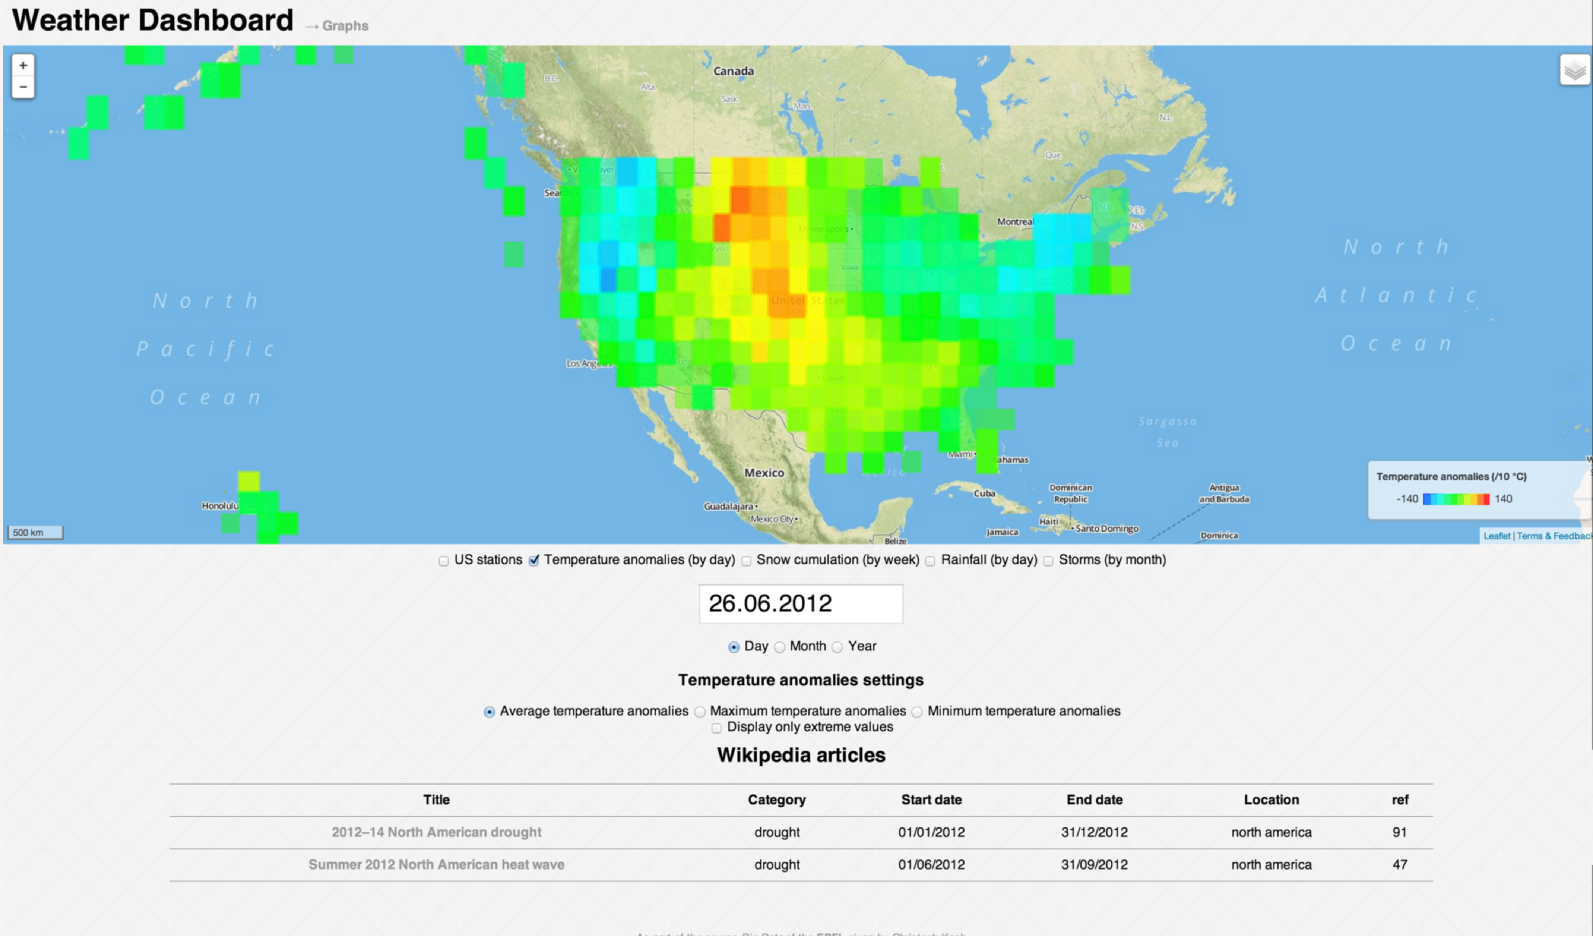
\includegraphics[scale=0.3]{figures/temperature}
   \caption{Example output of temperature anomalies on June, 26th 2012}
\end{figure}

We can clearly distinguish a wave of temperature hotter than the average for this period. Cells with more opacity and a bold contour have been classified as an extreme event.
These anomalies clearly corresponds to the wikipedia article displayed under the map.
